%% ----------------------------------------------------------------------
\chapter{Control target: WASP-18 b}
\label{ch:wasp18}

Before a pipeline is trusted with a new candidate, it should be run on a
planet whose answer is known. WASP-18~b (TIC~100100827) is a good choice: a
hot Jupiter of about 10 Jupiter masses on a 0.94-day orbit around a
$T_\mathrm{mag} = 8.8$ F6 star (Hellier et al.\ 2009), observed by TESS in
ten sectors between 2018 and 2026. The transit is 1~\% deep, and the planet
is so hot that TESS also sees it disappear behind the star: an
\emph{occultation} (secondary eclipse) of about 340~ppm at phase 0.5
(Shporer et al.\ 2019). A pipeline that validates WASP-18~b, finds its
occultation and does \emph{not} mistake that occultation for the sign of an
eclipsing binary, passes an honest test. This chapter shows that run and
what it taught us.

\section*{Set-up}
The profile \code{profile_WASP18b.json} (menu \emph{Profiles}) contains:
\begin{lstlisting}
"tic": "100100827", "outdir": "WASP18b",
"blind_search": true, "p_min": "0.5", "p_max": "10",
"ld_fit": true, "vet_neighbours": true, "sensitivity": true,
"red_noise_scrambles": "2000"
\end{lstlisting}
No period is given: the pipeline must find the planet itself with a blind
TLS search between 0.5 and 10~days. The run uses TESScut full-frame images
of sectors 2, 3, 29, 30, 69, 96, 103, 104, 105 and 106 (cadences 30, 10 and
3.3~min); the optimal apertures of 20--24 pixels contain 99.2--99.6~\% of the
target's light (Figure~\ref{fig:w18-field}). A complete run takes about two
hours, most of it in TRICERATOPS and the red-noise scrambles; the audit is
run afterwards with the button \emph{Audit}.

\begin{figure}[ht]
\centering
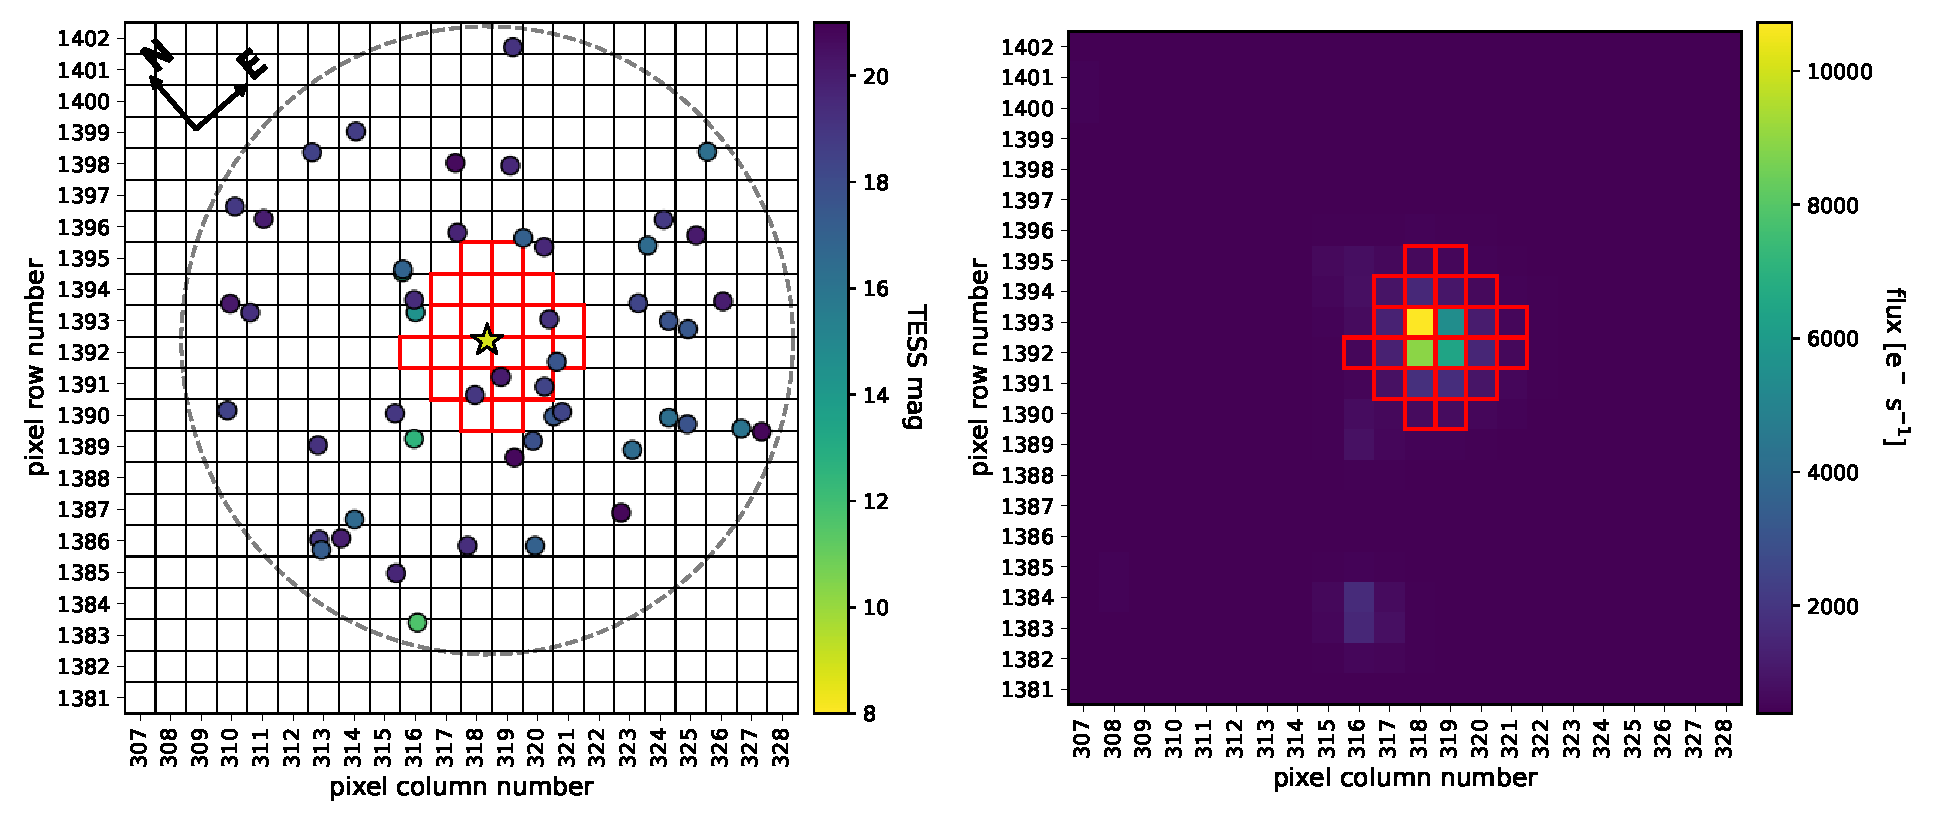
\includegraphics[width=0.85\textwidth]{wasp18_field_s104.pdf}
\caption{Sector 104: TIC stars on the TESS pixel grid (left) and the image
with the optimal aperture (right). WASP-18 is by far the brightest star in
the aperture.}
\label{fig:w18-field}
\end{figure}

\section*{Results}

\begin{longtable}{@{}p{0.33\textwidth}p{0.29\textwidth}p{0.30\textwidth}@{}}
\toprule
\textbf{Quantity} & \textbf{Pipeline} & \textbf{Literature}\\
\midrule\endhead
Period (blind search) & 0.941452~d (ETV fit) & 0.941452~d\\
Transits used & 257 in 10 sectors & ---\\
Duration T14 & 2.19~h & 2.2~h\\
Depth (limb-darkened fit) & 10\,938~ppm & ---\\
Depth (per-transit mean, adopted) & 10\,381 $\pm$ 9~ppm, $\chi^2_\nu = 1.4$ & ---\\
$R_p/R_\star$ & 0.0967 & 0.097\\
Impact parameter $b$ & 0.00 (at the fit limit) & $\approx$0.36\\
Stellar density from the transit & 1.05~g\,cm$^{-3}$ at $b = 0$ & ---\\
Planet radius (TP scenario) & 14.3~$R_\oplus$ = 1.28~$R_\mathrm{J}$ & $\approx$1.2~$R_\mathrm{J}$\\
Odd/even depths & 1.1$\sigma$ & ---\\
Secondary eclipse & phase 0.4985, 387~ppm, S/N 64 & phase 0.5, 341~ppm\\
Brightness temperature & $\approx$2900~K & dayside $\approx$3000~K\\
Timing (ETV) & O$-$C rms 0.7~min; no trend & ---\\
Difference imaging & on the target, median 0.1$\sigma$ (10 sectors) & ---\\
FPP / NFPP & 0 / 0 & ---\\
Verdict & PASSED & confirmed planet\\
\bottomrule
\end{longtable}

\begin{figure}[ht]
\centering
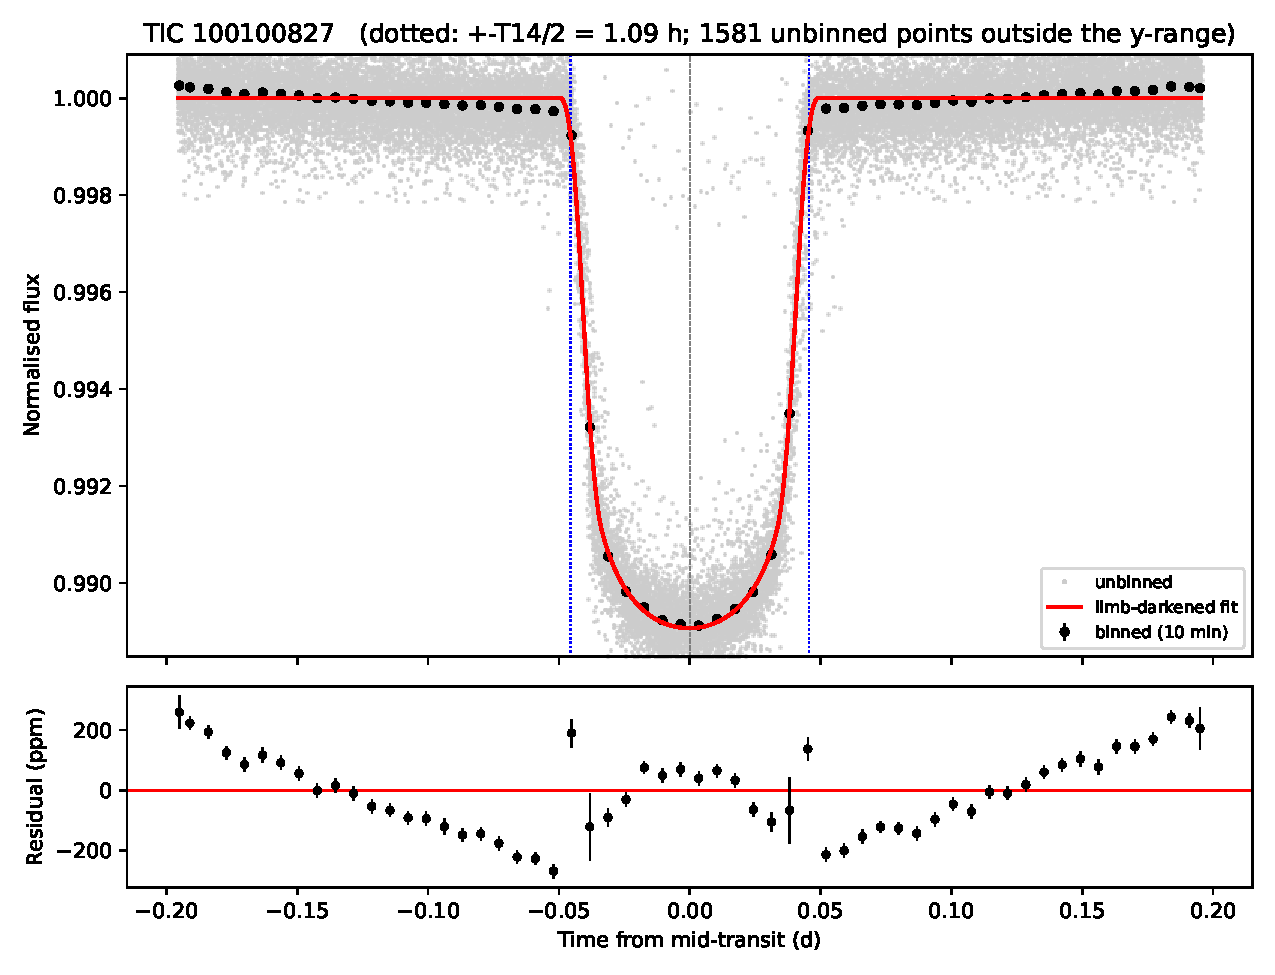
\includegraphics[width=0.49\textwidth]{wasp18_phased_transit.pdf}\hfill
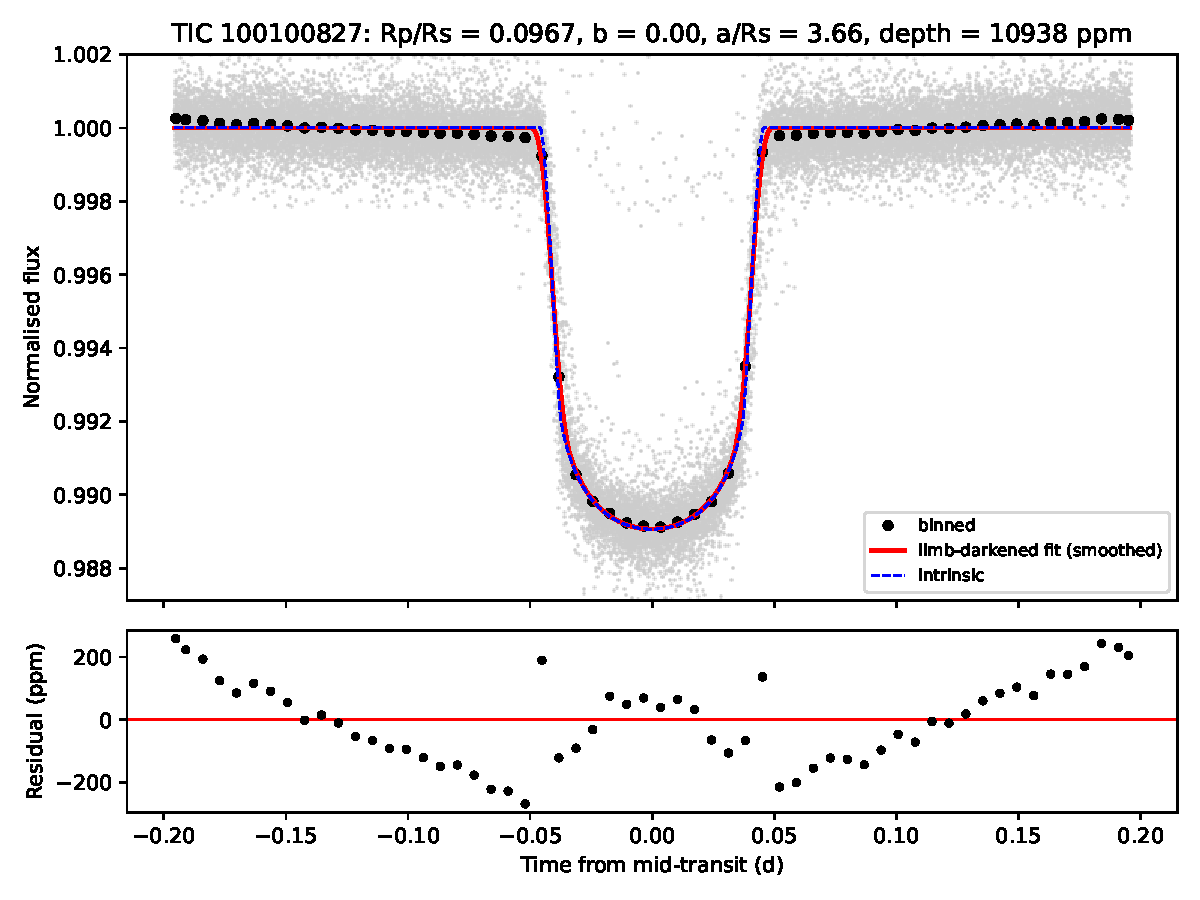
\includegraphics[width=0.49\textwidth]{wasp18_ld_fit.pdf}
\caption{Left: the 254 transits folded on the pipeline ephemeris, with the
limb-darkened fit and 10-min bins. Right: the limb-darkened fit on the
binned fold (smoothed with each sector's cadence). The residuals (lower
panels) are not flat: they show a wave of $\pm$250~ppm. That is not a
problem of the fit but a property of the star: the massive planet raises
tides on it, and its brightness changes twice per orbit (ellipsoidal
variation), on top of the planet's own phase curve.}
\label{fig:w18-transit}
\end{figure}

Two entries in the table deserve a comment.

\textbf{Impact parameter and density.} The fit puts $b$ at its lower limit
0, where the density of the star from the transit shape is
1.05~g\,cm$^{-3}$, against 0.69~g\,cm$^{-3}$ from the TIC mass and radius.
For a hot Jupiter with $R_p/R_\star \approx 0.1$ a central and a slightly
off-centre transit look almost the same in TESS data; the audit therefore
reports that ``$b$ is unconstrained and $b = 0.54$ gives the catalogue
density'', and the pipeline keeps its per-transit depth rather than the
limb-darkened one. The literature value $b \approx 0.36$ lies in between.
This is the normal situation for a deep, short transit; it is not a warning.

\textbf{Depth.} The depth passed to TRICERATOPS is the weighted mean of the
257 individual transits, 10\,381~ppm in the aperture; the limb-darkened fit
gives 10\,938~ppm at the bottom of the transit. Both describe the same
transit: the first is the mean over the box of the transit, the second its
deepest point.

\textbf{The noise used by TRICERATOPS.} The scatter of the binned fold
around the transit model is 160~ppm, while white noise alone would give
24~ppm. The difference is the ellipsoidal wave of
Figure~\ref{fig:w18-transit}. The pipeline uses the measured 160~ppm, which
is conservative: TRICERATOPS is told that the light curve is noisier than
its photon noise. This is why the sensitivity test (below) loses the pass
only when the noise is multiplied by four.

\begin{figure}[ht]
\centering
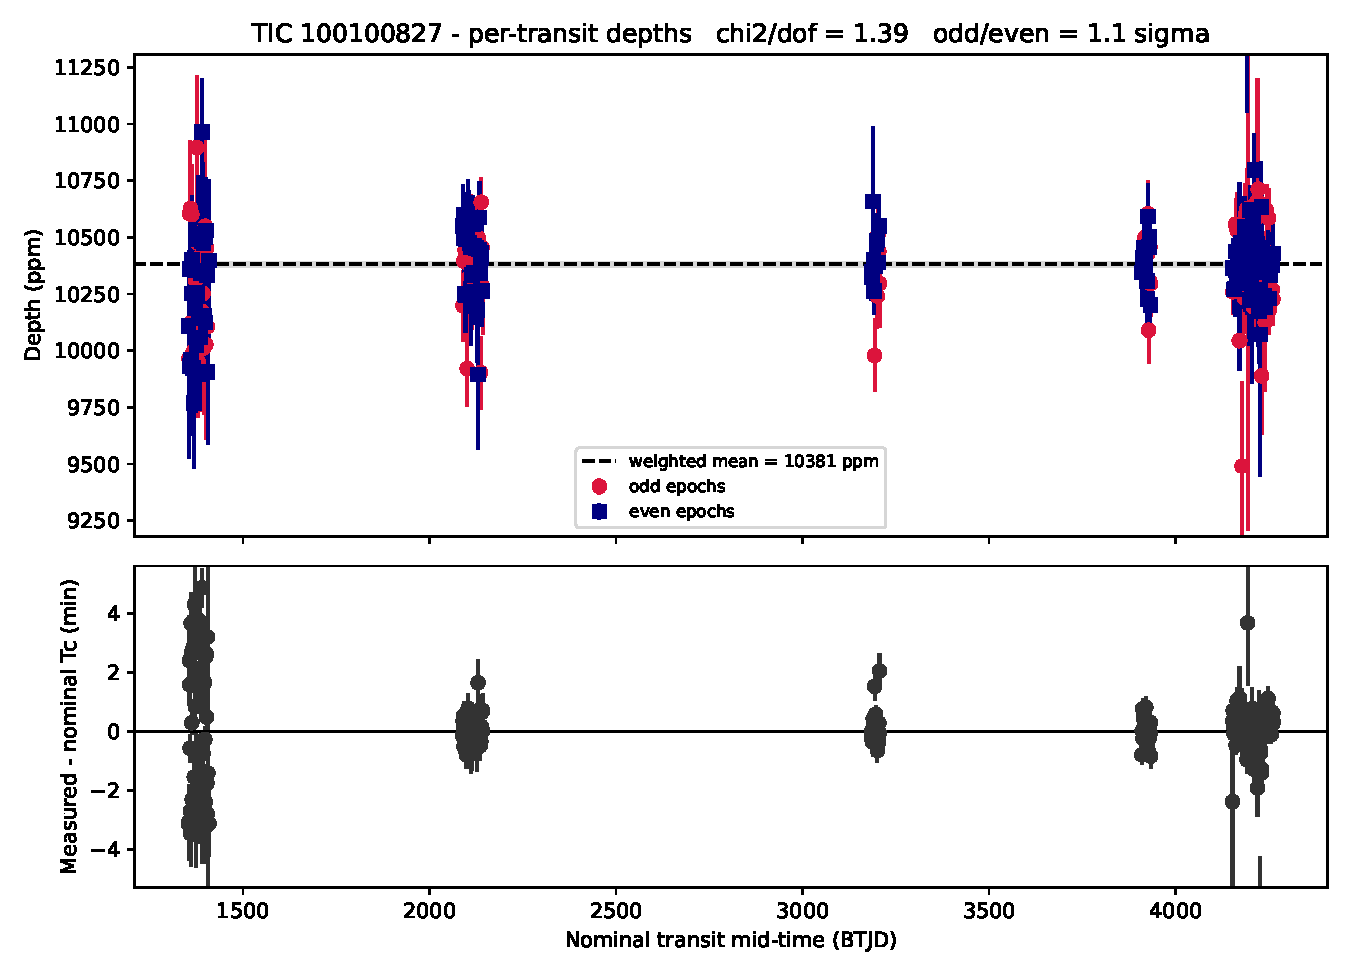
\includegraphics[width=0.62\textwidth]{wasp18_per_transit.pdf}
\caption{Depth (top) and mid-time offset (bottom) of the 257 individual
transits, measured with the trapezoid template. Odd (red) and even (blue)
transits agree (1.1$\sigma$); the depths scatter only 1.4 times their
errors over eight years; the mid-times agree with the linear ephemeris
within 1.3~min rms. The 30-min cadence of 2018 (left) gives the largest
scatter.}
\label{fig:w18-pt}
\end{figure}

\begin{figure}[ht]
\centering
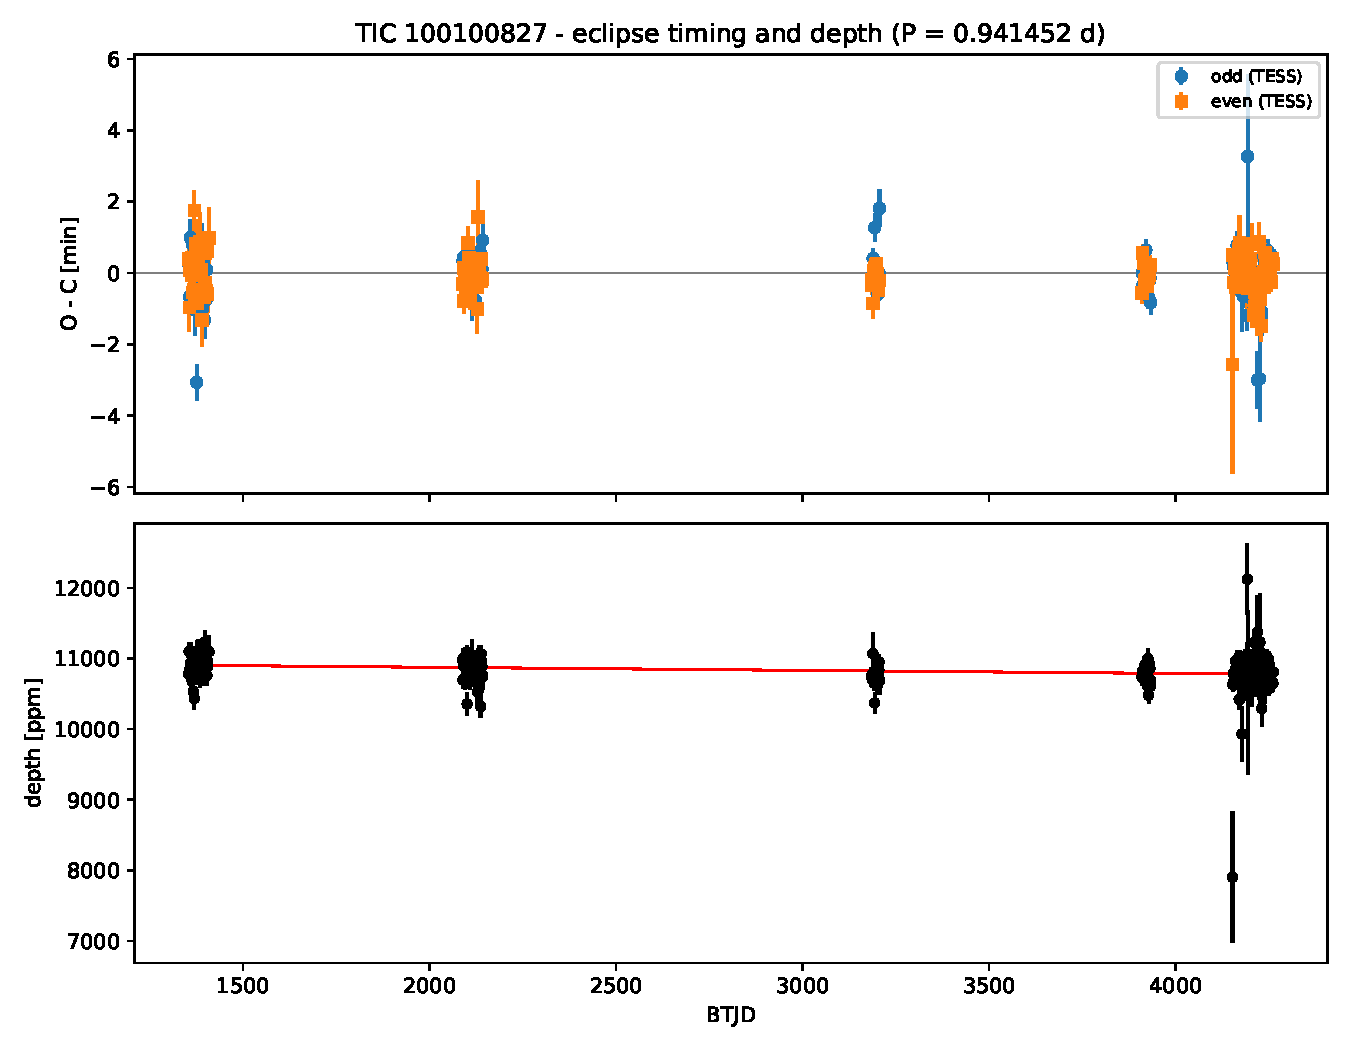
\includegraphics[width=0.62\textwidth]{wasp18_etv.pdf}
\caption{Eclipse timing (top) and depth (bottom) of 256 transits over eight
years. The mid-times scatter by 0.7~min around a constant period; there is
no sign of orbital decay or of a third body within the limits of TESS.}
\label{fig:w18-etv}
\end{figure}

\section*{The secondary eclipse}

The pipeline searches the whole orbit, not only phase 0.5, for a second dip
(Figure~\ref{fig:w18-sec}). For WASP-18 it finds one at phase 0.4985
(less than a minute from 0.5: a circular orbit), 387~ppm deep, with S/N 64
from 244 orbits. The depth ratio secondary/primary gives the surface
brightness of the second body in the TESS band, and from that a brightness
temperature of about 2900~K.

\begin{figure}[ht]
\centering
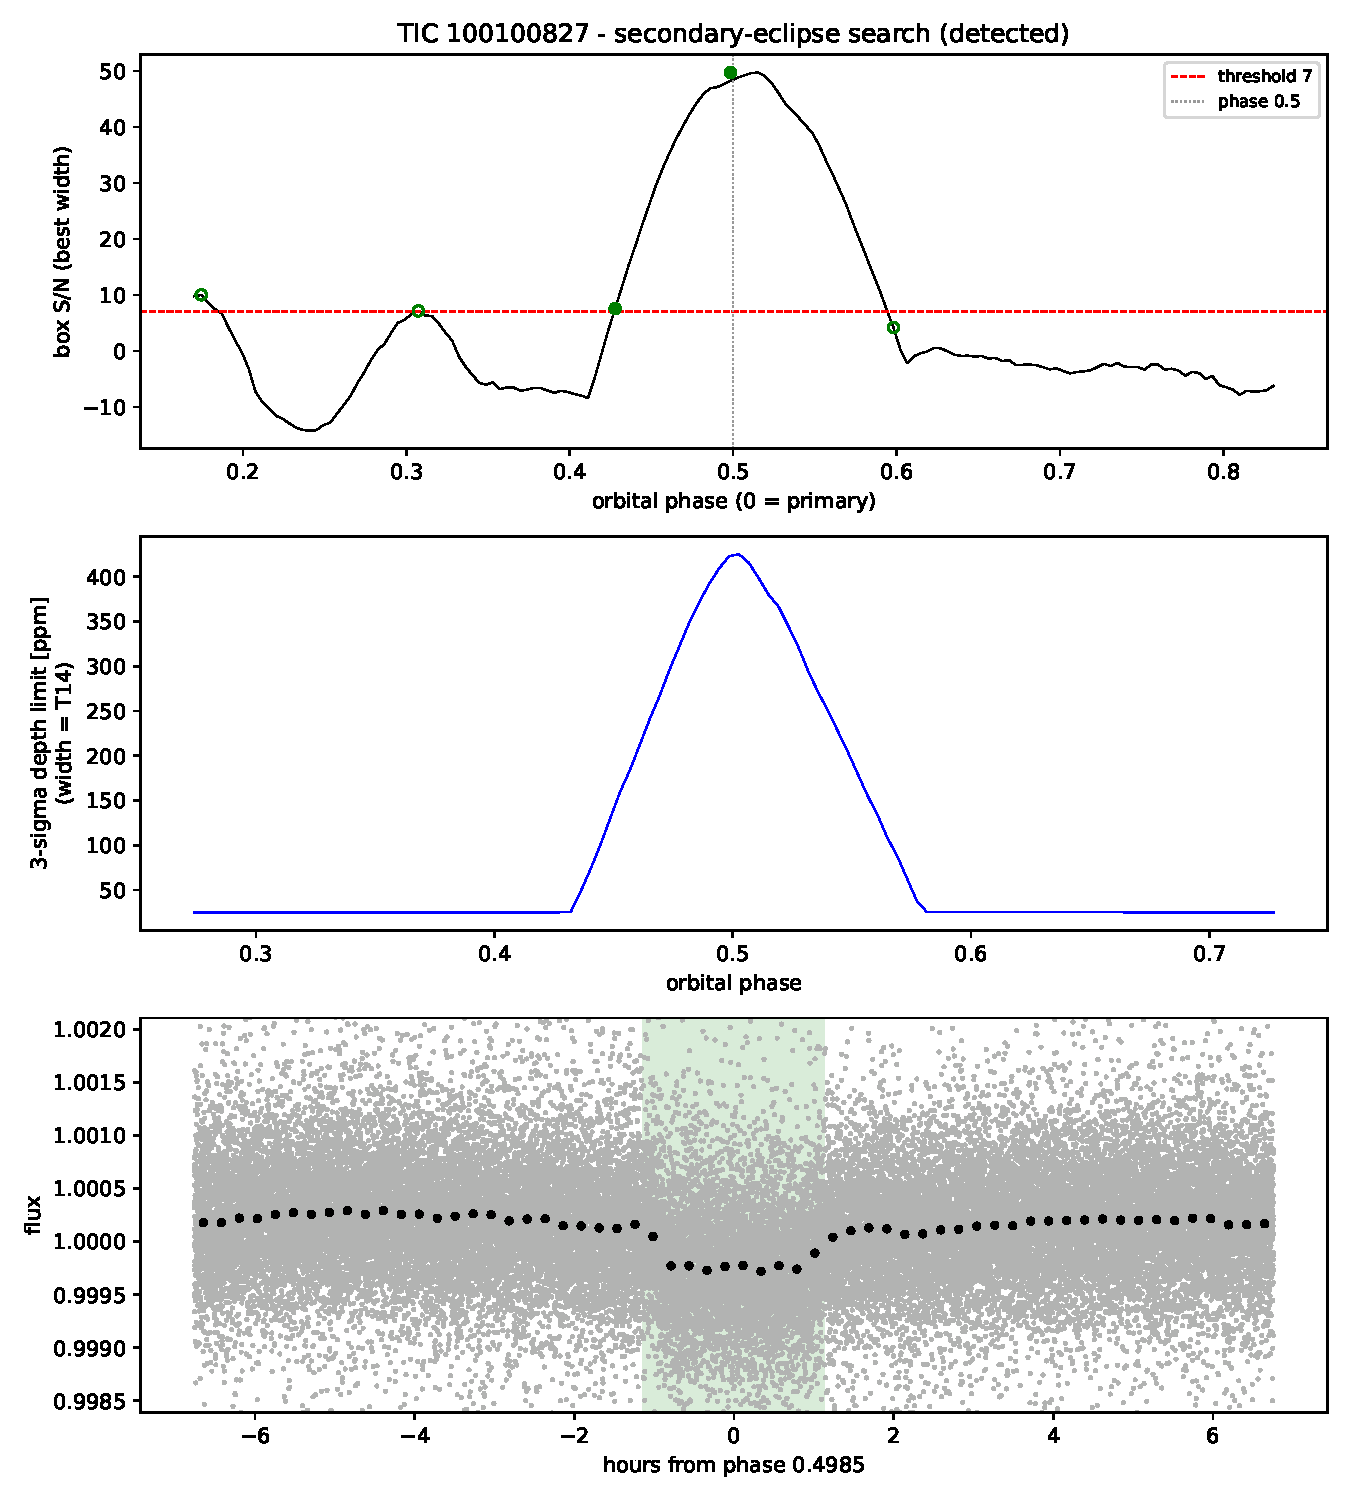
\includegraphics[width=0.7\textwidth]{wasp18_secondary_search.pdf}
\caption{Secondary-eclipse search. Top: S/N of a box search over the
orbital phase; the peak at 0.5 is the occultation. Middle: 3$\sigma$ depth
limit (near the primary no search is possible). Bottom: the light curve
folded on the secondary, with the eclipse window in green.}
\label{fig:w18-sec}
\end{figure}

A secondary eclipse is usually the strongest sign of an eclipsing binary.
Here it must not be: a planet at 2900~K also has a secondary eclipse.
The pipeline therefore applies a simple rule. A secondary eclipse that is
cooler than 4000~K \emph{and} less than 10~\% of the primary depth can be
the occultation of a hot planet; it is reported as a hint
(\code{eb_hints} in the summary) and is not used against the planet. A
self-luminous M dwarf of the same size would show the same signal, so the
audit lists it as a warning and states what decides: a radial-velocity
mass. For WASP-18~b that mass is known (10~$M_\mathrm{J}$): the warning is
correct, and the answer is ``planet''.

The measured 387~ppm is somewhat deeper than the published 341~ppm. The
pipeline measures the eclipse against a local baseline on both sides, and
on this star that baseline is bent by the phase curve; a full phase-curve
model, as in the literature, is beyond the purpose of a validation run.

\section*{Where the signal comes from}

With 99~\% of the light from WASP-18 and a 1~\% transit, the difference
image (out-of-transit minus in-transit) is bright and sharp in every sector
(S/N 1200--2650). Its centroid lies on the target to within 0.03~pixel; the
median offset over the ten sectors is 0.1$\sigma$
(Figure~\ref{fig:w18-di}). All 51 neighbours in the field are excluded as
the source.

\begin{figure}[ht]
\centering
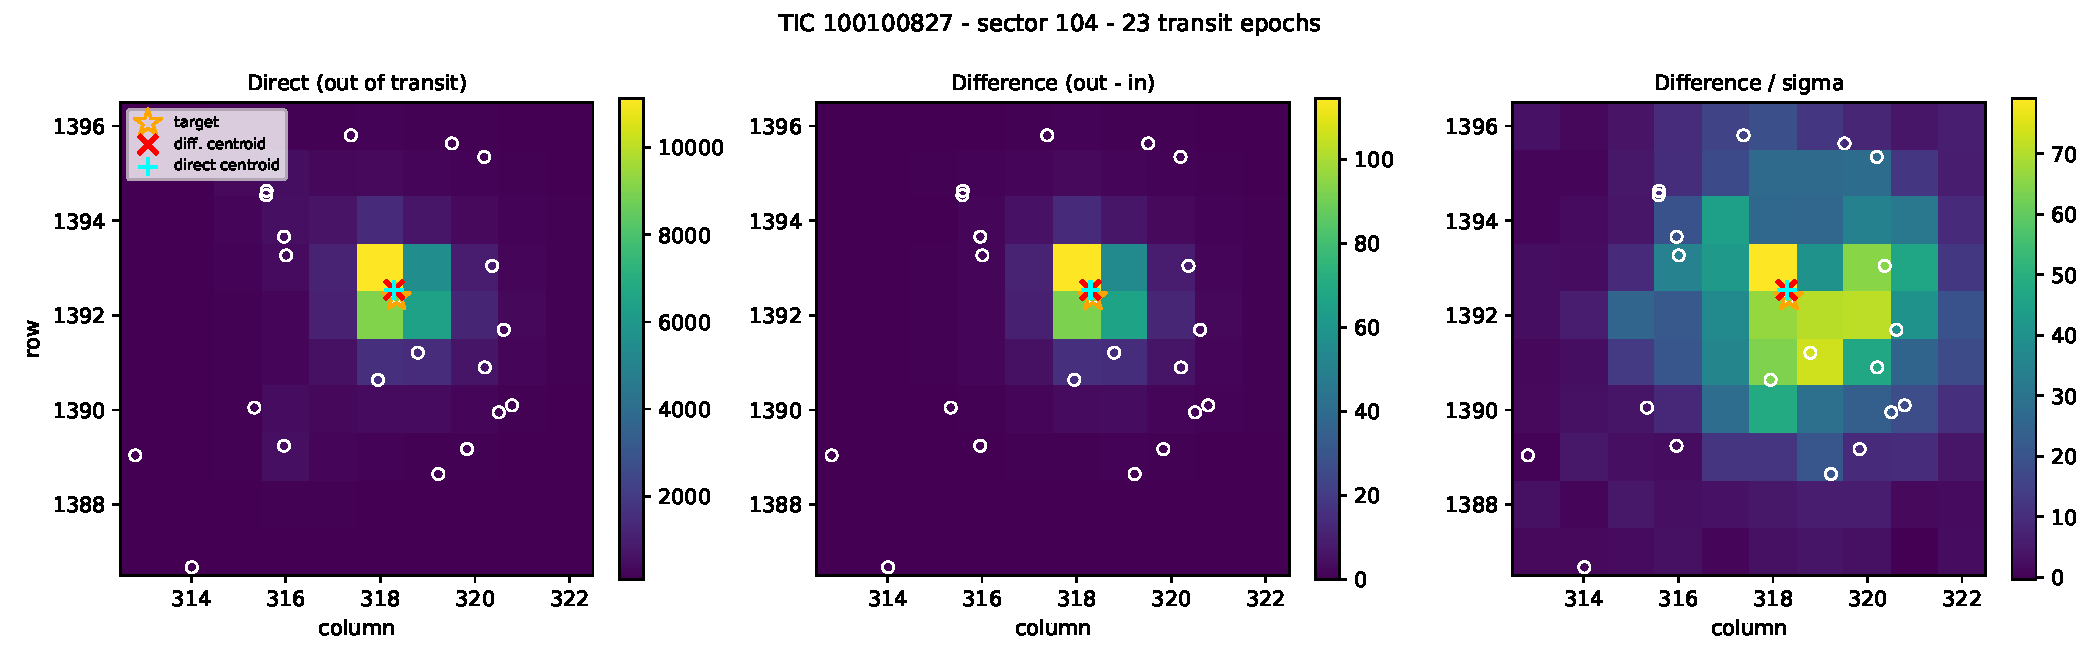
\includegraphics[width=\textwidth]{wasp18_diffimg_s104.pdf}
\caption{Difference imaging, sector 104: direct image (left), difference
image (middle) and difference divided by its error (right). Target, centroid
of the difference image and centroid of the direct image coincide.}
\label{fig:w18-di}
\end{figure}

\section*{TRICERATOPS, audit and next observations}

All 20 TRICERATOPS runs are valid. The probability goes entirely to the
planet scenarios: TP 0.87, PTP 0.07 (planet on the target, with an unseen
bound companion diluting it) and DTP 0.05 (the same with an unresolved
background star). Every other scenario has a probability below
$10^{-17}$: a 1~\% eclipse on a bright star, with a shape this well
measured, leaves no room for them. FPP and NFPP are both 0.

The sensitivity test repeats the calculation with the noise multiplied by
0.5, 2 and 4. The pass holds up to twice the measured noise
(FPP~0.004) and is lost only at four times (FPP~0.029); the audit records
this as a PASS, with the advice to report the table. The audit summary is:
\emph{no FAIL, 1 WARN} (the occultation), 12 PASS, 3 not applicable (no
input ephemeris, no ground data). The page \emph{Next observations} finds
nothing left to remove; for a new candidate of this kind it would point to
a radial-velocity measurement, the only observation that tells a hot
Jupiter from a low-mass star.

\begin{tip}
\textbf{Lessons from the control target.} WASP-18~b exposed four problems
in earlier versions of the pipeline, all fixed in v4.3:
(1)~the blind search used the 5$\times$ wider masking window to refine the
ephemeris: T0 was 4~h off, T14 came out as 9~h and the depth as 100~ppm,
and the fold showed a flat line --- \emph{if T14 or the depth of a known
planet look wrong, suspect the ephemeris first};
(2)~the audit counted every secondary eclipse as a failure, also the
occultation of a hot planet;
(3)~the phase curve pulled the secondary eclipse to phase 0.52;
(4)~in sectors with strong scattered light the difference image had
S/N~$<1$ until bad frames were removed;
(5)~the template for the individual transits came from the TLS search on
binned data and was misaligned: the mid-times were biased by 10--17~min
and the adopted depth by $-9$ to $+9$~\%. The template is now the
trapezoid fitted to the fold on the adopted ephemeris
(Figure~\ref{fig:w18-pt}: mid-times within 1.3~min rms).
Run WASP-18~b again after every change to the pipeline: it takes two
hours, and the answer is known.
\end{tip}
